\chapter{Concept and Implementation} \label{sec:cha3}

The five inductors discussed in this chapter, listed in table \ref{tab:list_of_inductors}, are all products produced by the manufacturer Coilcraft. Falling under the category of power inductors, they are designed to be used in \ac{SMPS} and are therefore common in buck converters. Inductors with similar inductances and core materials were chosen to remain comparable to each other.
\begin{table}[H]
    \centering
    \caption{List of Inductors}
    \begin{tabular}{|c|c|l|}
    \hline
    Inductor &  Inductance & Type \\
    \hline
     XGL1313-103ME & $10 \mu H$ & Molded Inductor \\
        XGL1313-223ME & $22 \mu H$ & Molded Inductor \\
        SER1512-103ME & $10 \mu H$ & High Current Flat Wire Inductor \\
        SER1512-223ME & $22 \mu H$ & High Current Flat Wire Inductor \\
        UA8014-AL & $2 \cdot 10 \mu H$ & Uncoupled Dual Inductors \\
    \hline
    \end{tabular}
    \label{tab:list_of_inductors}
\end{table}

\section{Frequency Response of the Inductor} \label{sec:frequency_response_of_the_inductor}
The first and simplest type of inserting non-idealities into the inductor Model of LTspice is with an \ac{ECM} simulating the frequency response of a real inductor. The base inductor already has an \ac{ECM} pictured in figure \ref{fig:inductor_ecm}. It takes into account the equivalent parallel capacitance between the individual windings of the inductor $EPC$, the copper resistance at low frequencies $ESR$ and the overall resistance during resonance $EPR$. It acts as a starting point to approximate the frequency response of an inductor and as later demonstrated, is enough to characterise the above-mentioned inductors frequency response fully.
\begin{figure}[H]
    \centering
    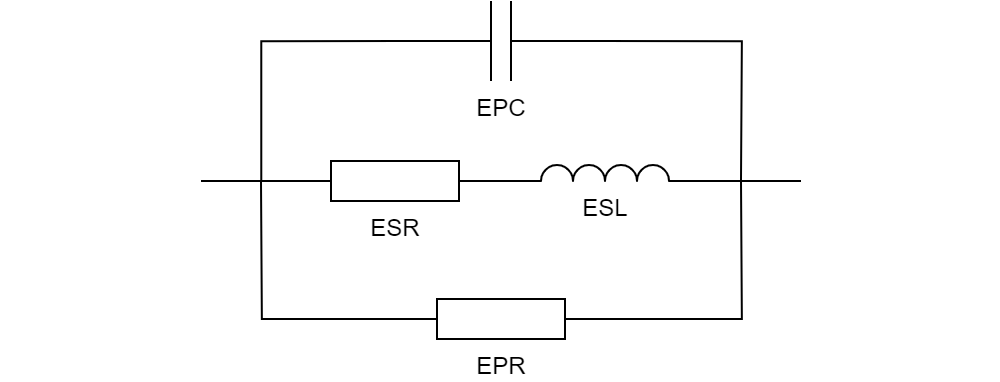
\includegraphics[width=0.75\linewidth]{Bilder//Kapitel3/Inductor_ECM.png}
    \caption{Inductor \ac{ECM}}
    \label{fig:inductor_ecm}
\end{figure}
To accurately measure the inductors frequency response a "Bode 100" by omicron-lab was used. It functions by subjecting the device under test to a sinusoidal frequency sweep from \SI{1}{\Hz} to \SI{50}{\mega\Hz} and measuring its scattering parameters for every frequency. With this data gain, phase, inductance and \ac{Q-factor} are plotted as dashed lines in figure \ref{fig:bode_100_measurements}. Starting out close to purely resistive, the plot shows a shift to inductive behaviour at around \SI{10}{\kilo\Hz}, with magnitude increasing proportional to frequency and the phase approaching \SI{90}{\degree}. At the point of resonance, there is once again a short moment of pure resistive behaviour, after which the inductor begins to act like a capacitor, its magnitude decreasing and phase reaching \SI{-90}{\degree}.\\
\begin{figure}[]
    \begin{subfigure}[b]{0.50\textwidth}
        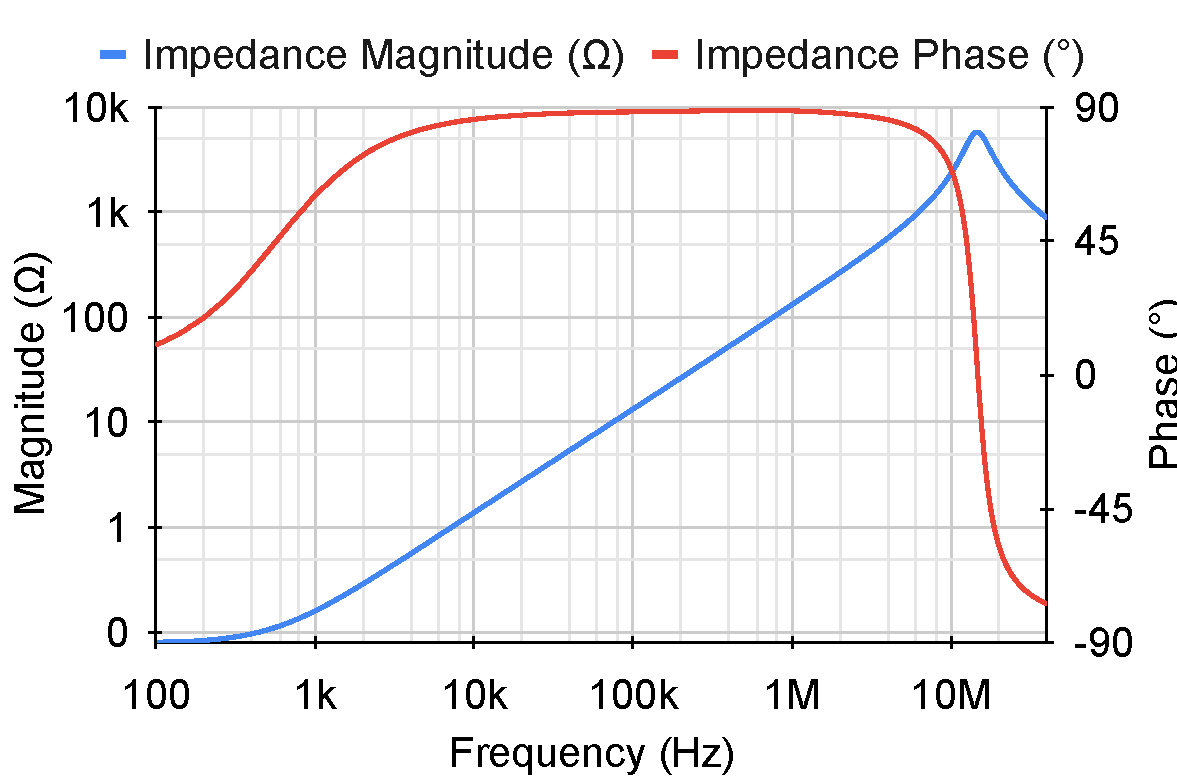
\includegraphics[width=\textwidth]{Bilder/Kapitel3/SER223_BodePlot.pdf}
        \caption{SER1512-223ME complex magnitude and phase vs frequency}
    \end{subfigure}
    \begin{subfigure}[b]{0.50\textwidth}
        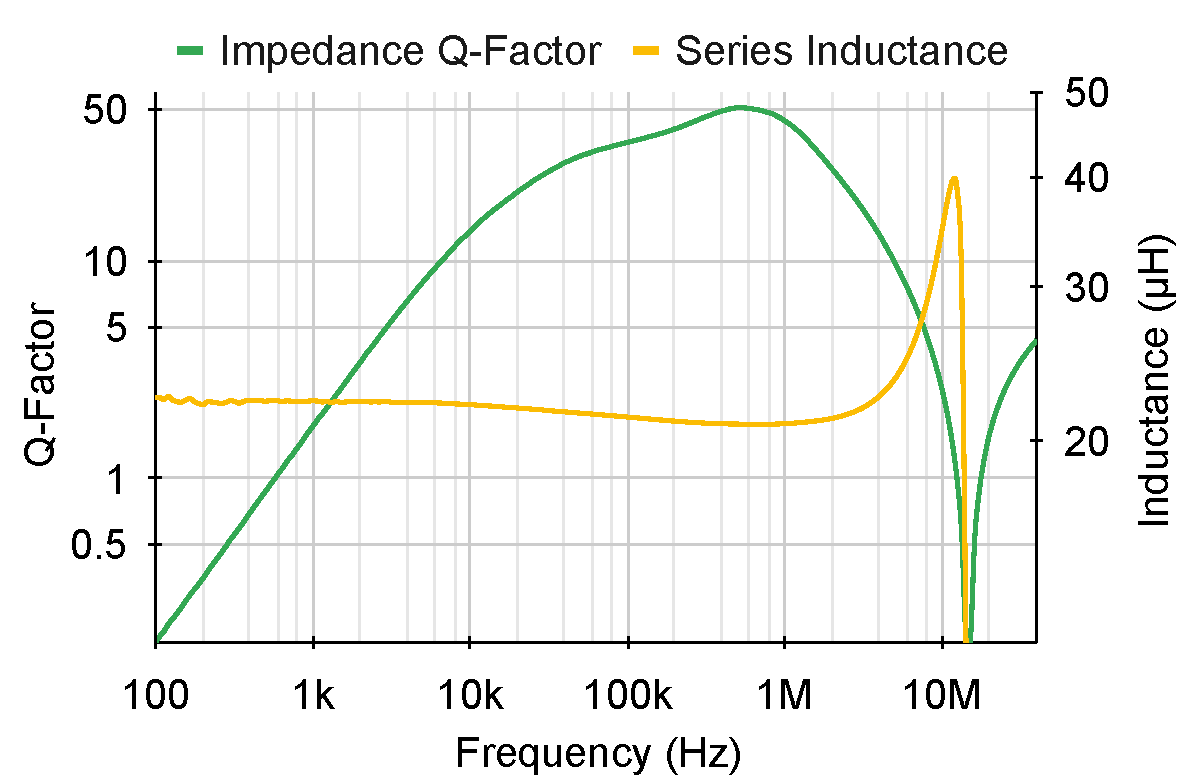
\includegraphics[width=\textwidth]{Bilder/Kapitel3/SER223_QLPlot.pdf}
        \caption{SER1512-223ME \ac{Q-factor} and inductance vs frequency}
    \end{subfigure}
    \caption{Measured frequency response of the SER1512-223ME}
    \label{fig:bode_100_measurements}							
\end{figure}
Applying this the inductance and series resistance can simply be read from the two graphs at the lowest available frequency. While for this inductor, the phase at this point still isn't zero and therefore inductive properties remain, the approximation still holds true, as both magnitude and phase level out before this point. Parallel capacitance and resistance are determined by the point of resonance. For this inductor, the resonant point lies at \SI{14,725}{\mega\Hz} with a pure resistance of \SI{5,582}{\kilo$\Omega$}. This resistance defines the parallel resistance of the \ac{ECM}. As resonance happens at the point, where the inductive reactance and capacitive reactance are equal, the capacitance can be determined by
\begin{equation}\label{eq:ecm_capacitance}
    C_P = \frac{1}{\left(2 \pi \cdot f_r\right)^2\cdot L} \quad\text{.}
\end{equation}
With this, all parameters for the \ac{ECM} can easily be determined.\\
Simulating the frequency response in LTspice is done by connecting the inductor model to a current source set to \ac{AC} analysis, with an amplitude of \SI{1}{A}. Measuring the voltage across the entire equivalent circuit after running an \ac{AC} simulation yields the frequency response of the inductor. Since the amplitude and phase of the voltage are determined by the product of the frequency-dependent impedance and the current, which is always \SI{1}{A} with a \SI{0}{\degree} angle, the complex measured voltage value equals the responding impedance value $Z_L$ at that frequency. The \ac{Q-factor} gives insight into how well the inductor is approximating an ideal inductor, showing a range for the optimal operating frequency for the inductor considering pure sinusoidal excitation. It is calculated by
\begin{equation}
    Q = \frac{Im(Z_L)}{Re(Z_L)} \quad\text{.} 
\end{equation}
The inductance simply is the imaginary part of the impedance up until resonance, as after that the inductor behaves like a capacitor. 
\begin{figure}[H]
    \begin{subfigure}[b]{0.50\textwidth}
        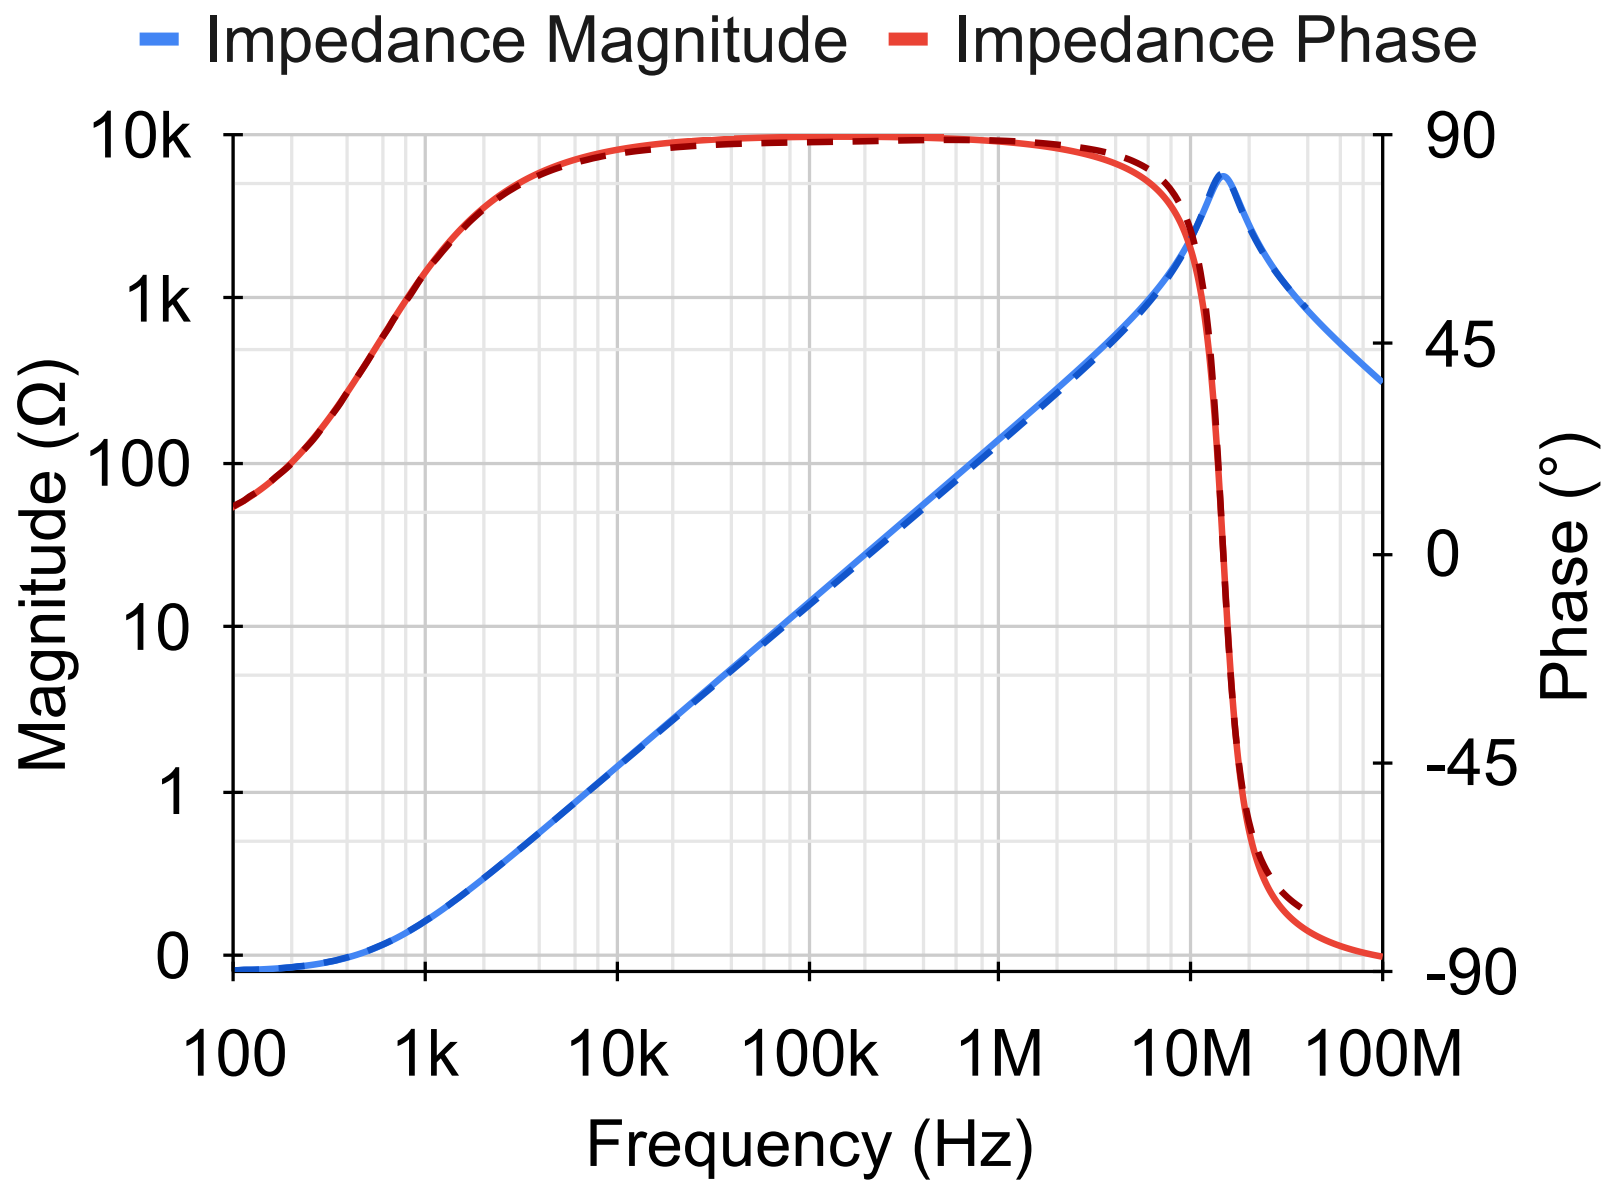
\includegraphics[width=\textwidth]{Bilder/Kapitel3/SER223_BodePlot_Combined.png}
        \caption{SER1512-223ME complex magnitude and phase vs frequency}
    \end{subfigure}
    \begin{subfigure}[b]{0.50\textwidth}
        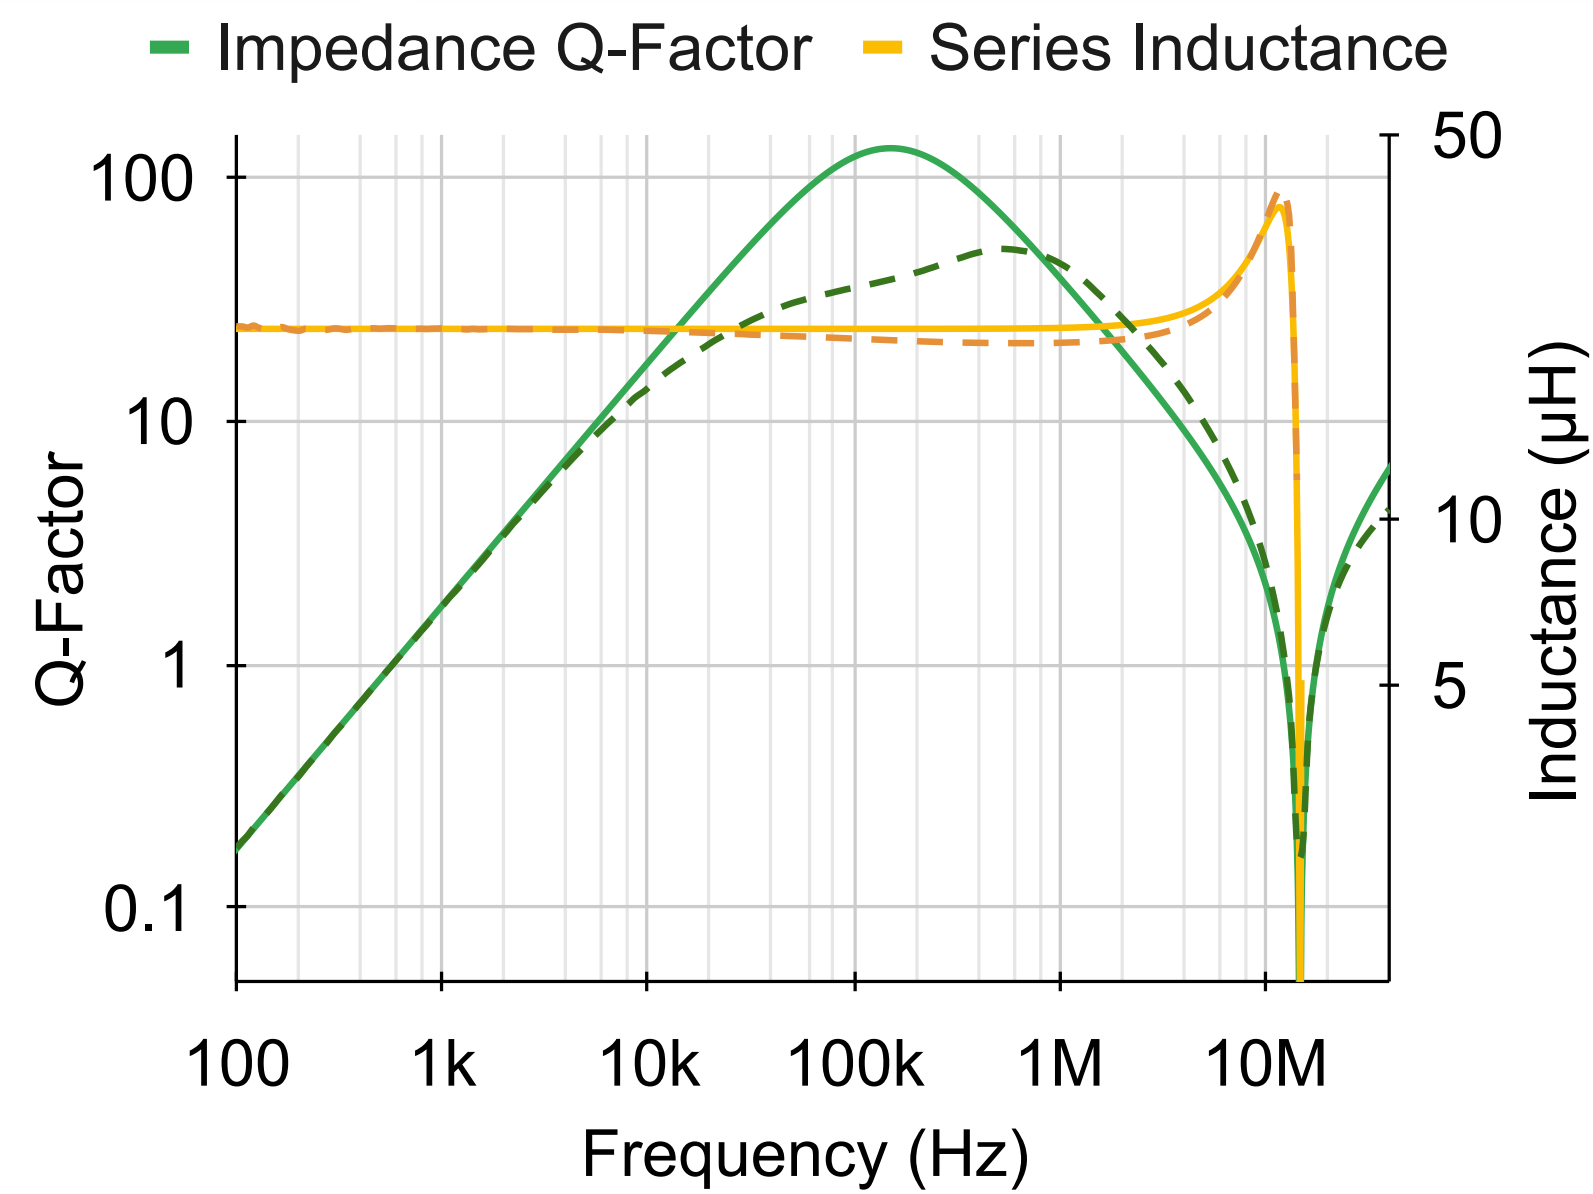
\includegraphics[width=\textwidth]{Bilder/Kapitel3/SER223_QLPlot_Combined.png}
        \caption{SER1512-223ME \ac{Q-factor} and inductance vs frequency}
    \end{subfigure}
    \caption{Simulated and measured frequency response of the SER1512-223ME\\striped lines indicate measured values, while continuous lines are simulated}
    \label{fig:bode_100_measurements_combined}							
\end{figure}
Overlaying the results of the measurements and the LTspice simulation in figure \ref{fig:bode_100_measurements_combined}, the \ac{ECM} closely models the true frequency response, justifying its use. While impedance magnitude and phase match close to perfectly, the \ac{Q-factor} and inductance slightly stray from the true values. Since the \ac{Q-factor} is sensitive to small changes in the imaginary part of the impedance its deviation from the measurement can be attributed to the slight frequency dependence of the measured inductance. The small change of the inductance before resonance is not separately modeled in the simulation \ac{ECM}, leading to the error in the \ac{Q-factor}.
Using this approach, all five inductors were modelled and implemented in LTspice with similar results to the ones presented. The results of figure \ref{fig:bode_100_measurements} show, that the frequency response of the simulated inductor is able to fully recreate the frequency behaviour of the physical inductor.
\begin{figure}[H]
   \begin{subfigure}[b]{0.50\textwidth}
       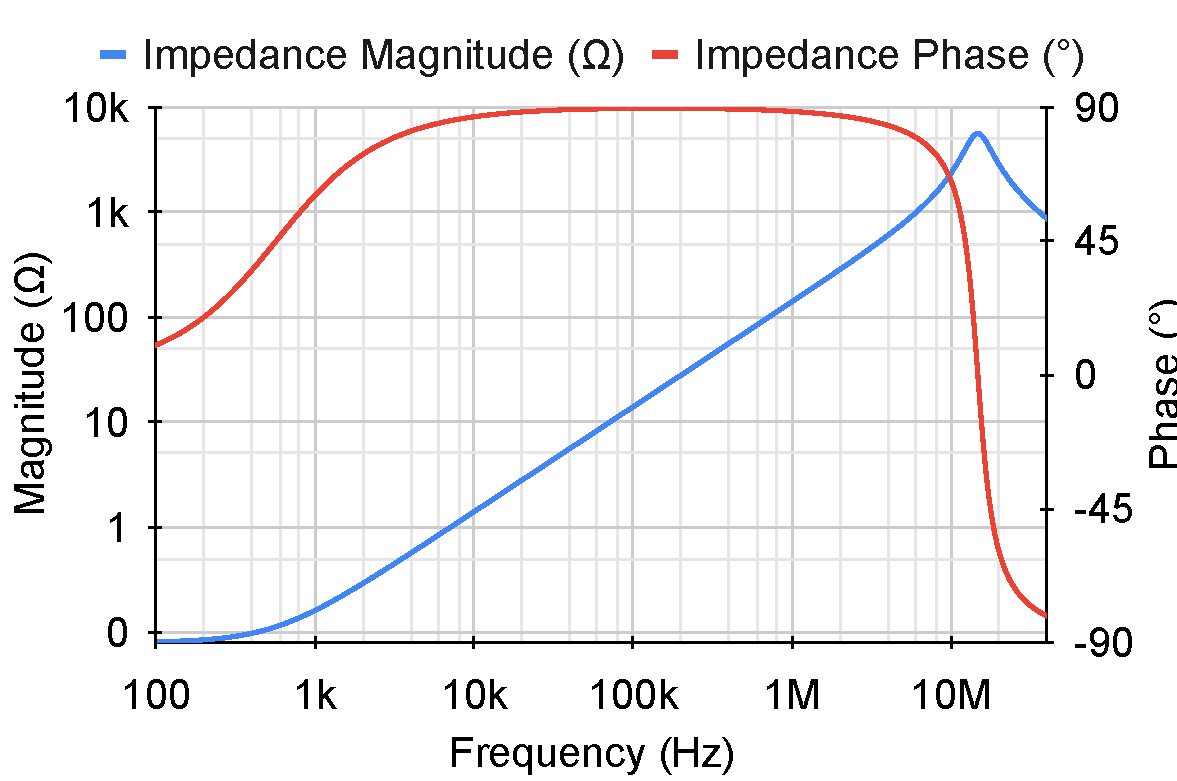
\includegraphics[width=\textwidth]{Bilder/Kapitel3/SER223_BodePlot_Spice.pdf}
       \caption{SER1512-223ME complex magnitude and phase vs frequency}
   \end{subfigure}
   \begin{subfigure}[b]{0.50\textwidth}
       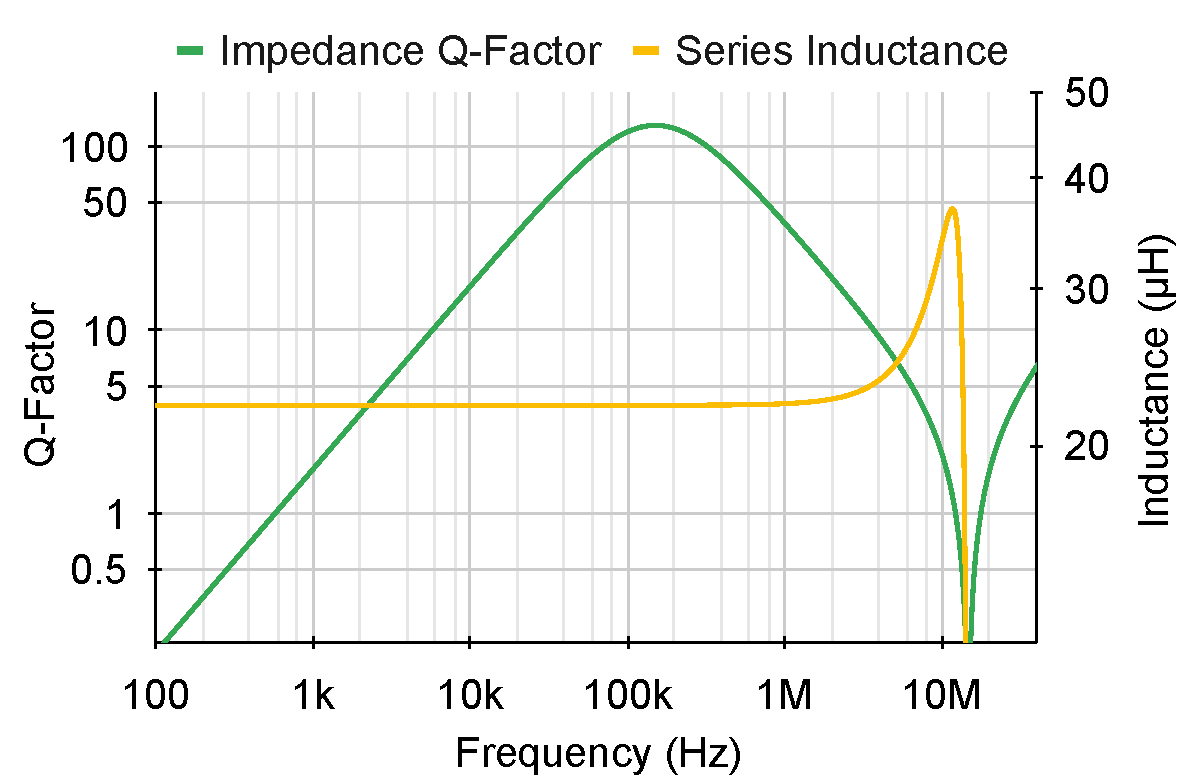
\includegraphics[width=\textwidth]{Bilder/Kapitel3/SER223_QLPlot_Spice.pdf}
       \caption{SER1512-223ME Q-factor and inductance vs frequency}
   \end{subfigure}
   \caption{Result of the LTspice simulation}
   \label{fig:LTspice_Frequency_Response}
\end{figure}

Quelle:https://www.omicron-lab.com/products/vector-network-analysis/bode-100/technical-data
\newpage
\section{Saturation Behaviour of the Inductor}\label{sec:saturation_behaviour_of_the_inductor}
The second type of inductor loss modelling takes advantage of the LTspice inbuilt \textit{flux} function. With it a  specific saturation curve can be input into the inductor, modelling the current dependence of the inductance. Since this model does not influence the frequency behavior of the inductor, it should be used in combination with the results from section \ref{sec:frequency_response_of_the_inductor}. \\
\subsection{Measuring the Saturation Behaviour}
To measure the saturation behaviour a "Power Choke Tester" by the manufacturer ed-k was used. It subjects the inductor under test to a rectangular voltage pulse and measures the current through it until a set maximum current is reached. The voltage applied is set to be similar to the actual voltage the inductor is subjected to, here set to \SI{30}{V}. With the voltage and current data, the device is able to calculate the magnetic flux in the inductor. Calculating the saturation behaviour is done by differentiating the flux.\\ 

The measured saturation behaviours of the \textit{SER1512-223ME}, \textit{UA8014-AL} and \textit{XGL1313-103ME} inductors is displayed in figure \ref{fig:differential_inductance_of_the_ser1512-223me_inductor}. Considering the \textit{SER1512-223ME} inductor, a close to constant inductance with an average of \SI{21.8}{\micro\henry} can be measured up to a current of \SI{5}{\A}, after which the curve decreases following an s-curve. Levelling out at an inductance around \SI{1.18}{\micro\henry}. This means that the inductor enters saturation at around \SI{5}{\A} of \ac{DC} through it, marking this current as the maximum current the inductor should experience without causing the ripple current to increase, resulting in greater power losses.
\begin{figure}[h]
    \centering
    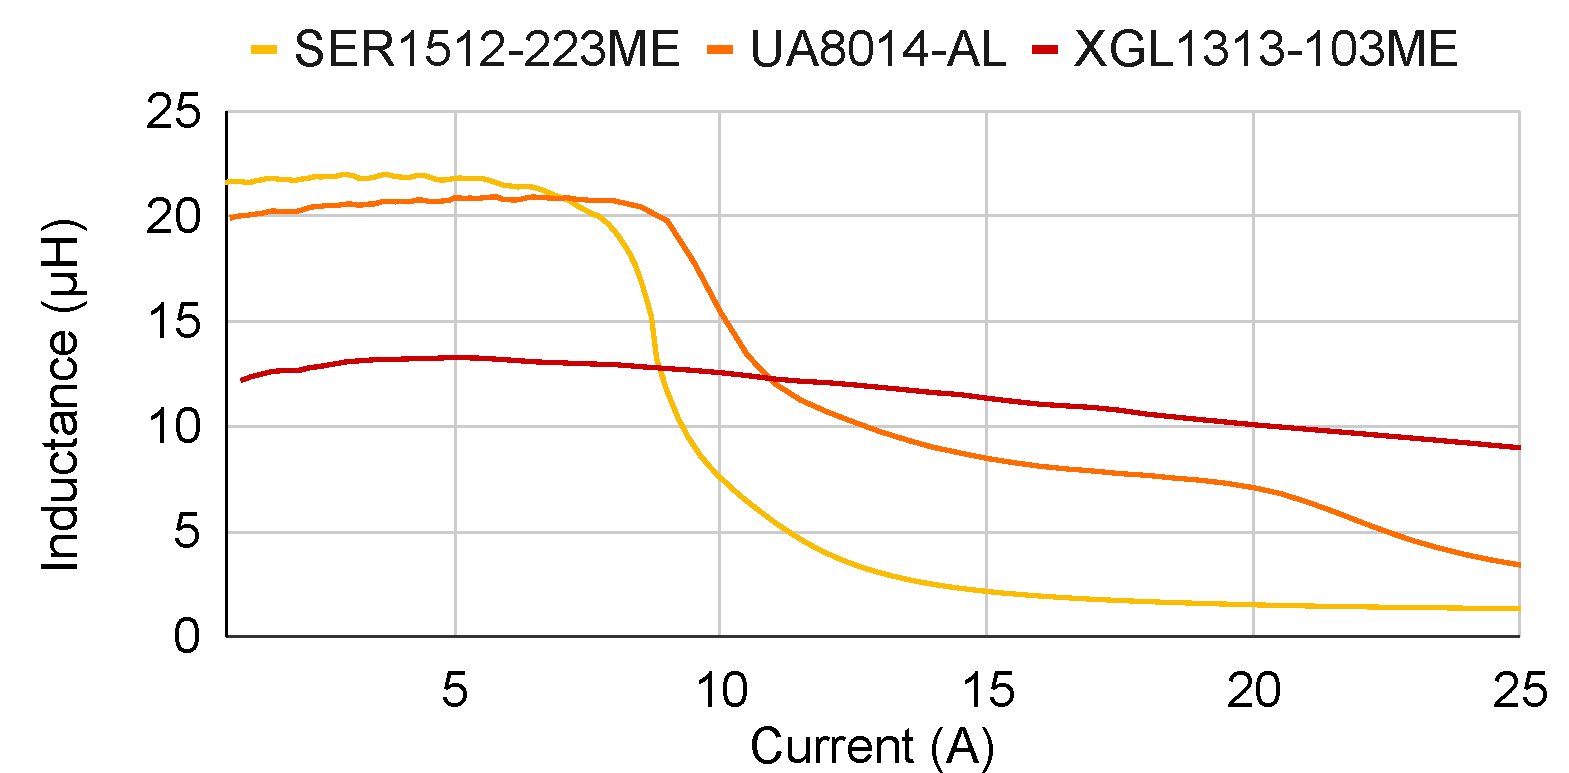
\includegraphics[width=0.8\linewidth]{Bilder//Kapitel3/SER223_UA_XGL103_Saturation.pdf}
    \caption{Differential inductance of the SER1512-223ME and UA8014-AL inductor}
    \label{fig:differential_inductance_of_the_ser1512-223me_inductor}
\end{figure}
The difference in behaviour of this inductor to the \textit{XGl1313-103ME} inductor can be lead back to two reasons. Firstly the \textit{XGL}-inductor is only a \SI{10}{\micro\H} inductor, compared to the \SI{22}{\micro\H} \textit{SER}-inductor. This explains why their inductances outside of saturation are so different. Secondly, the very gradual reduction of the saturation of the \textit{XGL}-inductor can be traced back to its core material. Being made from composite materials, instead of a ferrite, the inductor has an effective air gap, that is spread throughout the entire core. Large air gaps soften the transition into saturation and increase the saturation current. \\
\subsection{Simulating the Saturation Behaviour}
To represent the current behaviour of the inductance in the simulation, the measured data needs to be imported. Directly importing the measured flux value by value into LTspice is no option, as both the number of values LTspice is able to store is limited and the runtime of the simulation is drastically increased. Instead, curves are fitted to the saturation measurements that best describe the inductance for each inductor. A combination of different degree polynomials and exponential functions define a piecewise function that approximates the saturation behaviour of the inductance. Integrating this function yields the flux curve, which can then be imported into LTspice using the \textit{flux}-command of the inductor.\\
Measuring the inductance curve in the simulation is done by subjecting the inductor to an \ac{AC} with an amplitude of $\frac{1}{2\pi}$\SI{ }{\A}, frequency of \SI{1}{\Hz} and a varying \ac{DC} offset. The chosen amplitude and frequency enable the inductance to be determined by measuring the voltage across the inductor. As the inductors voltage is the product of the \ac{AC} amplitude and the inductors complex impedance, the frequency factor of $2\pi$ and the currents amplitude cancel out, resulting in the voltage being numerically equivalent to the inductance.
\begin{equation}\label{eq:inductance_from_voltage}
    \hat{V}_L = \hat{I}_L \cdot j 2\pi f\cdot L \triangleq L
\end{equation}

Comparing the inductance curve of the \textit{UA8014-AL} inductor when measured and simulated, the flexibility and precision of this approach can be well demonstrated. The fitted curve consisting of many piecewise defined functions is able to closely follow the measured inductance. While sensibly extending the inductance curve up to \SI{0}{\A} of current, high frequency measurement noise visible in the low amperage range of the measured inductance curve is also removed. Furthermore it has the advantage of causing no noticeable increase to the simulation runtime when compared to a model not taking advantage of the \textit{flux}-command. 
\begin{figure}[H]
    \centering
    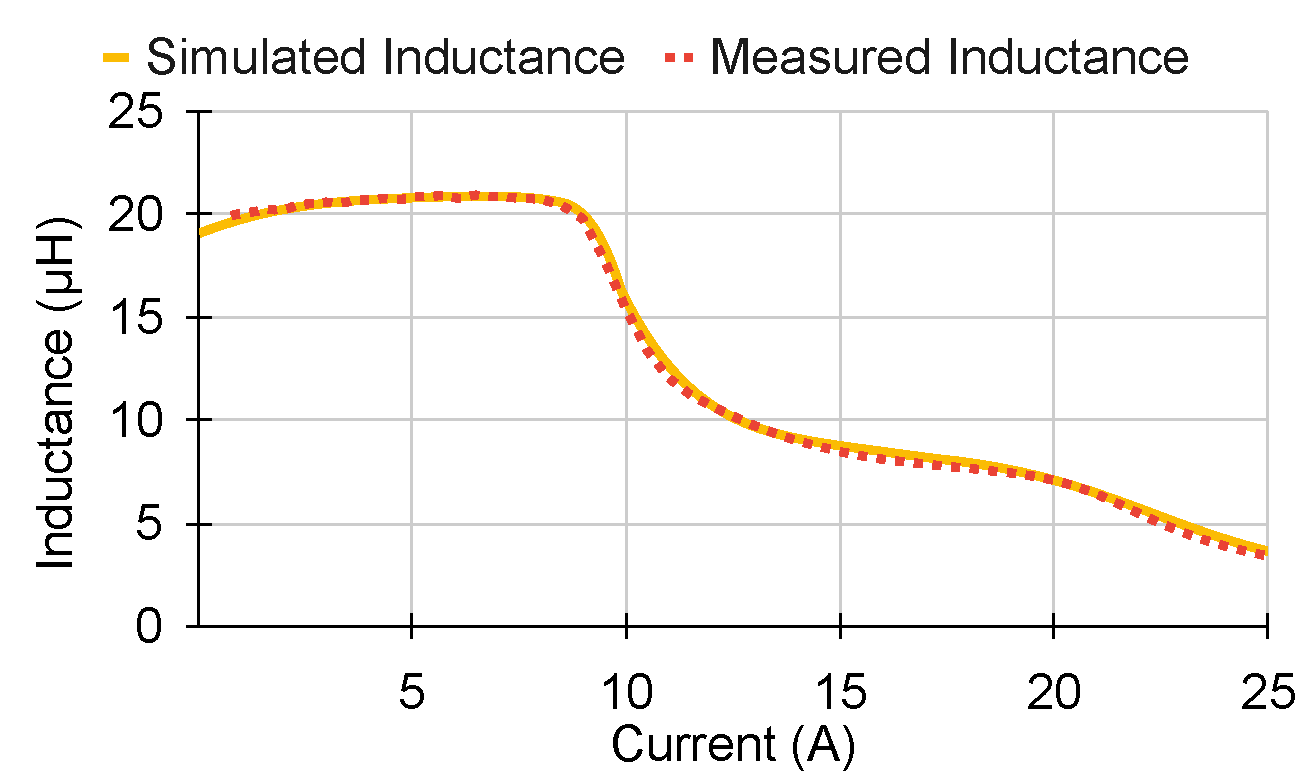
\includegraphics[width=0.7\linewidth]{Bilder/Kapitel3/Saturation_Measured_vs_LTspice.pdf}
    \caption{Comparison of the Inductance curve of the \textit{UA8014-AL} measured and simulated}
    \label{fig:comparison_of_saturation}
\end{figure}

\newpage
\section{Hysteresis Behavior of the Inductor} \label{sec:hysteresis_behaviour_of_the_inductor}
The third type of inductor modelling provided by LTspice is hysteresis modelling. In contrast to the saturation model, it takes the \ac{DC} bias into account with the hope of modeling the inductor behaviour at high output currents accurately.\\
In contrast to the flux, where a function can be directly input in LTspice, the hysteresis curve is defined via seven parameters: 
\begin{table}[H]
    \centering
    \caption{LTspice hysteresis modeling parameters}
    \begin{tabular}{|c|c|}
        \hline
        $N$ & Number of turns\\
        \hline
        $l_m$ & Length of magnetic core\\
        \hline
        $l_g$ & Length of air gap\\
        \hline
        $A_c$ & Crossectional area \\
        \hline
        $B_{max}$ & Maximum B-field\\
        \hline
        $B_r$ & Remnant B-field\\
        \hline
        $H_c$ & Coercivity\\
        \hline
    \end{tabular}
    \label{tab:ltspice_hystersis_modling_parameters}
\end{table}
 The last three of these directly define the shape of the hysteresis curve, while the others are needed to calculate the inductance based on the hysteresis. As for many inductors, among others all inductors used in this thesis, these parameters are not provided by the inductor manufacturer, it is necessary to measure the hysteresis curve.
 \subsection{Measuring the Hysteresis of a Custom Inductor}
 To provide a proof of concept for the hysteresis measurement and simulation, a custom inductor is created with known core parameters. The chosen core from the producer ferroxcube, called PQ20/16 \cite{ferroxcubeMaterialSpecifications3C952015, ferroxcubeProductSpecificationsCore2016}, came with exact values for each of the hysteresis modeling parameters and a measured hysteresis curve. This provides a validation of the measurement approach and eliminates errors in the measurement of the cores dimensions. The core is wound with 8 windings and pressed together to create an inductor without an air gap. Hereby all variables for the hysteresis measurement are known.
\begin{table}[H]
    \centering
    \caption{Parameters of the custom inductor \cite{ferroxcubeMaterialSpecifications3C952015}}
    \begin{tabular}{|l|c|c|c|c|}
        \hline
        Parameter & Magnetic length $l_m$ &  Air gap length $l_g$ &  Effective area $A_e$ & Windings $N$ \\
        \hline
        Value & \SI{37.8}{\milli\m} & \SI{0}{\milli\m} & \SI{61.9}{\milli\square\m} & 8\\
        \hline
    \end{tabular}
    \label{tab:parameters_of_the_custom_inductor}
\end{table}
 Measuring the hysteresis is done by subjecting the inductor under test to a rectangular voltage pulse until the core reaches saturation. After that the voltage is dropped and the inductor discharges on its own. Since there was no dedicated device available, the setup displayed in figure \ref{fig:hysteresis_measurement_setup} needed to be implemented manually.
\begin{figure}[H]
    \centering
    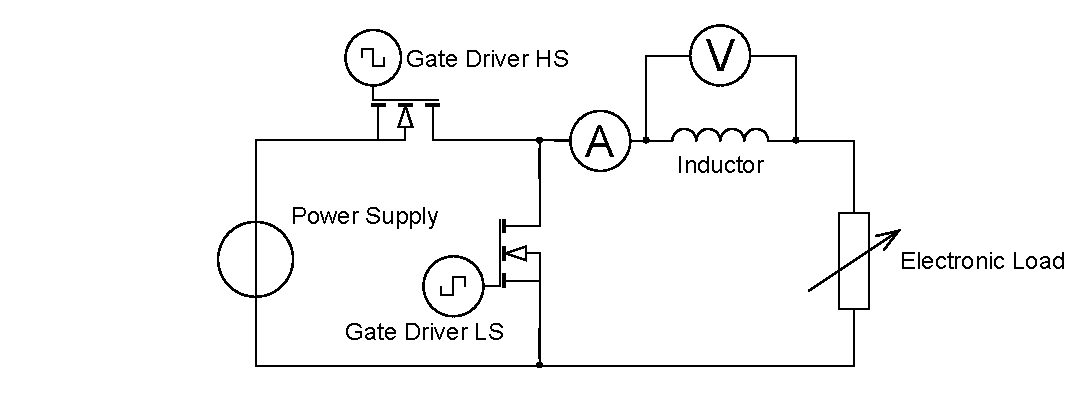
\includegraphics[width=1\linewidth]{Bilder/Kapitel3/Hysteresis_Measurement_Setup.pdf}
    \caption{Hysteresis measurement setup}
    \label{fig:hysteresis_measurement_setup}
\end{figure}
Using a \ac{GaNFET} half-bridge to connect the inductor to and adding a load with capacitive and resistive properties, allows the charging time to be regulated and a reverse current to flow through the inductor. The reverse current is necessary to measure the coercive force $H_c$. Connecting a current clamp to the wire leading to the inductor and a voltage probe across the inductor enables the oscilloscope to measure the B-H curve. As the voltage supplied to the inductor determines the rate of change of the inductor current, a lower switching frequency is desirable, as it allows a lower voltage to be used to achieve the same maximum current, since more time for the charging process is given.\\
Limiting factors of this setup are the minimum speed the \ac{GaNFET} half-bridge can switch at, the maximum change in current the power supply can deliver and the maximum power spikes the electronic load is able to handle. In this case the minimum switching speed achieved was \SI{10}{\kilo\Hz}, which is just low enough to enable a clear measurement.\\
%The main limiting factor of this setup is the minimum speed the \ac{GaNFET} half-bridge can switch at. Being designed for high switching speeds, up from \SI{100}{\kilo\Hz}, comes with the downside of not being able to properly switch at \SI{10}{\kilo\Hz}, as the capacitor holding the charge to enable the gate to switch will discharge too quickly.  The selected power source however not only has to supply this voltage but also be able to handle rapid changes in the supplied current. This limits the power sources available. Concerning the connected load, it has to be able to handle the great power spikes created. Furthermore the resistive load has to be small enough to allow the desired current to flow, as the maximum voltage is set by the power source.\\

The here used Tektronix Series 6 oscilloscope comes with a inbuilt function to directly measure a B-H curve. Achieving the proper scale of the B-H curve requires adding the number of turns, crossectional area and magnetic length into the settings of the oscilloscope. \\

Inserting the custom inductor into the measurement setup shown in figure \ref{fig:hysteresis_measurement_setup}, applying a \SI{52}{\V} supply voltage, allowing a maximum \SI{30}{\A} current pull and switching at \SI{13}{\kilo\Hz}, the behaviour shown in image \ref{fig:hysteresis_measurement_of_the_custom_wound_inductor} was created. 
Hysteresis and saturation behaviour are clearly visible. However, the noise at the points where the axes are crossed is substantial, influencing the values of the remnant B-field $B_r$ and the coercivity $H_c$. Most of this noise is most likely measurement noise, as the oscilloscope needs to measure high voltages and currents, which worsens the resolution at low currents and voltages. The distortion visible at the maximum point of saturation is due to fluctuations in the voltage of the power supply, as it operates at its peak capabilities.
\begin{figure}[H]
    \centering
    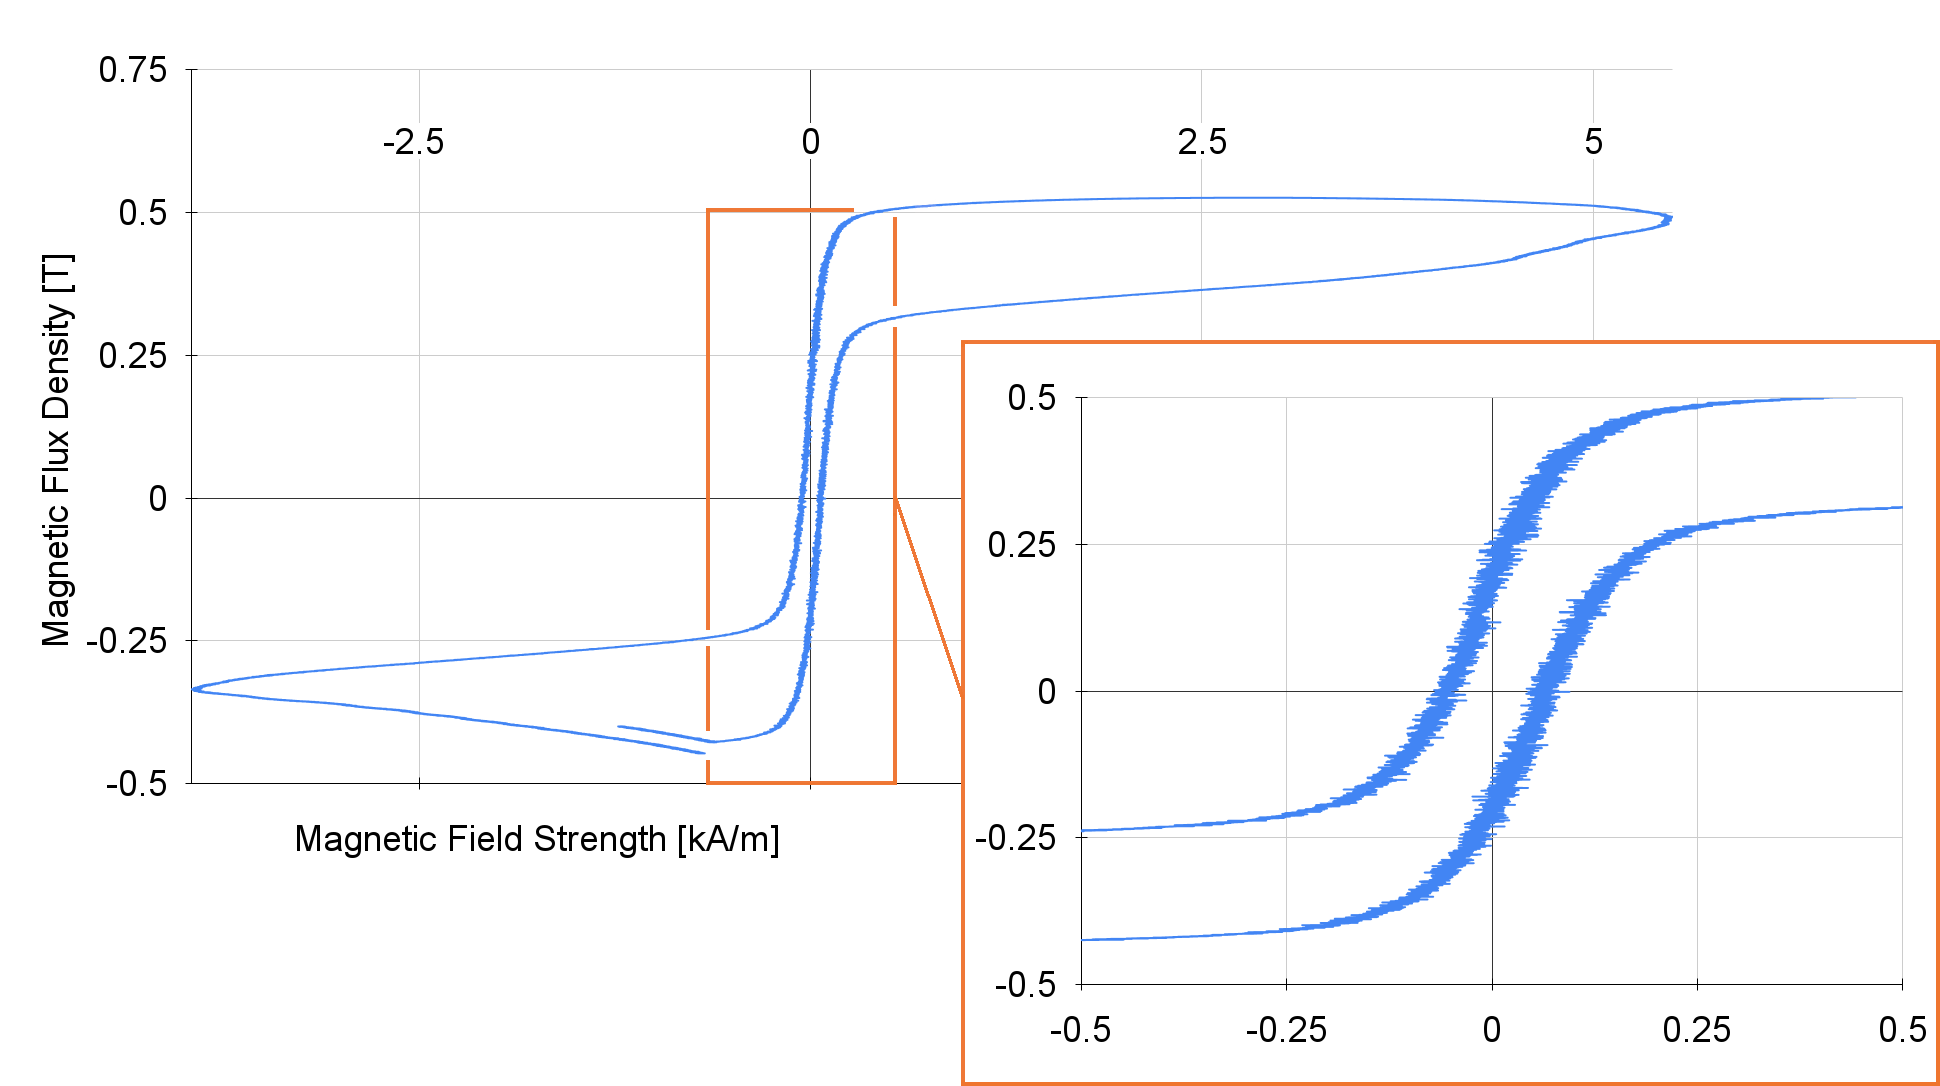
\includegraphics[width=1\linewidth]{Bilder//Kapitel3/Hysteresis_Measurement_3.png}
    \caption{Hysteresis Measurement of the custom wound inductor}
    \label{fig:hysteresis_measurement_of_the_custom_wound_inductor}
\end{figure}
Table \ref{tab:B-H_curve_points_of_interest_comparison} compares the measured points of interest to the data provided by the producer of the core material. While the deviations are significant, they are still attributable to the noise and limitations of the setup. If the setup is changed to allow for higher precision at low currents and voltages and the saturation region is not plagued by unwanted behaviour of the power supply and electronic load, the results can be improved. This validates the use of this approach to also measure inductors, who's core parameters are unknown. 
\begin{table}[H]
    \centering
    \caption{Comparison of B-H curve parameters \cite{ferroxcubeProductSpecificationsCore2016}}
    \begin{tabular}{|l|c|c|}
        \hline
        & Measured & Given by the data sheet \\
        \hline
        Coercive Force $H_c$ & \SI{54}{\A\per\m} & \SI{13}{\A\per\m}\\ 
        \hline
        Remnant B-Field $B_r$ & \SI{255}{\milli\tesla} & \SI{156}{\milli\tesla}\\
        \hline
        Maximum B-Field $B_{max}$ & \SI{570}{\milli\tesla} & \SI{500}{\milli\tesla}\\
        \hline
    \end{tabular}
    \label{tab:B-H_curve_points_of_interest_comparison}
\end{table}
Knowing that the B-H curve is measurable and that its results, after appropriate changes to the setup, should match reality, the implementation in LTspice is now discussed.
\subsection{Simulation of the Hysteresis of a Custom Inductor}
To ensure that the use of ideal values in the LTspice simulation results in the desired behaviour and provides a representative model, the B-H curve is simulated purely with the values given by the cores data sheet, listed in table \ref{tab:parameters_of_the_custom_inductor} and table \ref{tab:B-H_curve_points_of_interest_comparison}. \\
Verifying the LTspice simulation is done by plotting the B-H curve of the simulated inductor. For this a sinusoidal current is applied to the inductor with no \ac{DC} bias and at the same frequency as the data sheet uses, \SI{10}{\kilo\Hz}. The B- and H-field values are calculated through Faraday's and Amperes law. Faraday's law states, that a changing magnetic flux $\Phi$ induces a voltage in a wire loop with the cross-sectional area $A$. As the magnetic flux can be expressed as the product of the area $A$ and the magnetic flux density $B$ and the voltage is proportional to the number of loops of wire $N$, the equation can be rearranged to 
\begin{equation}\label{eq:faradays_law}
	B = \frac{1}{N \cdot A} \int_0^t u(\tau)d\tau \quad\text{.}   
\end{equation}
In contrast, Ampere's law describes that the magnetic field $H$ integrated along a closed loop is equal to the current enclosed by this loop. As in the core of an inductor, the magnetic field can be assumed to be constant and the length of the loop is given by the magnetic length $l_m$ of the core, the integral can be resolved. As the core encloses $N$ windings of the coil, the current creating the magnetic field is equal to the supplied current $I$ times the number of windings. Solving for the magnetic field, results in 
\begin{equation}\label{eq:amperes_law}
	H = I \cdot \frac{N}{l_m} \quad\text{.}
\end{equation}
Using behavioural voltage and current sources, the equations \ref{eq:faradays_law} and \ref{eq:amperes_law} can be directly implemented in LTspice, as they allow for functions and integration. The complete setup is seen here. 
\begin{figure}[H]
    \centering
    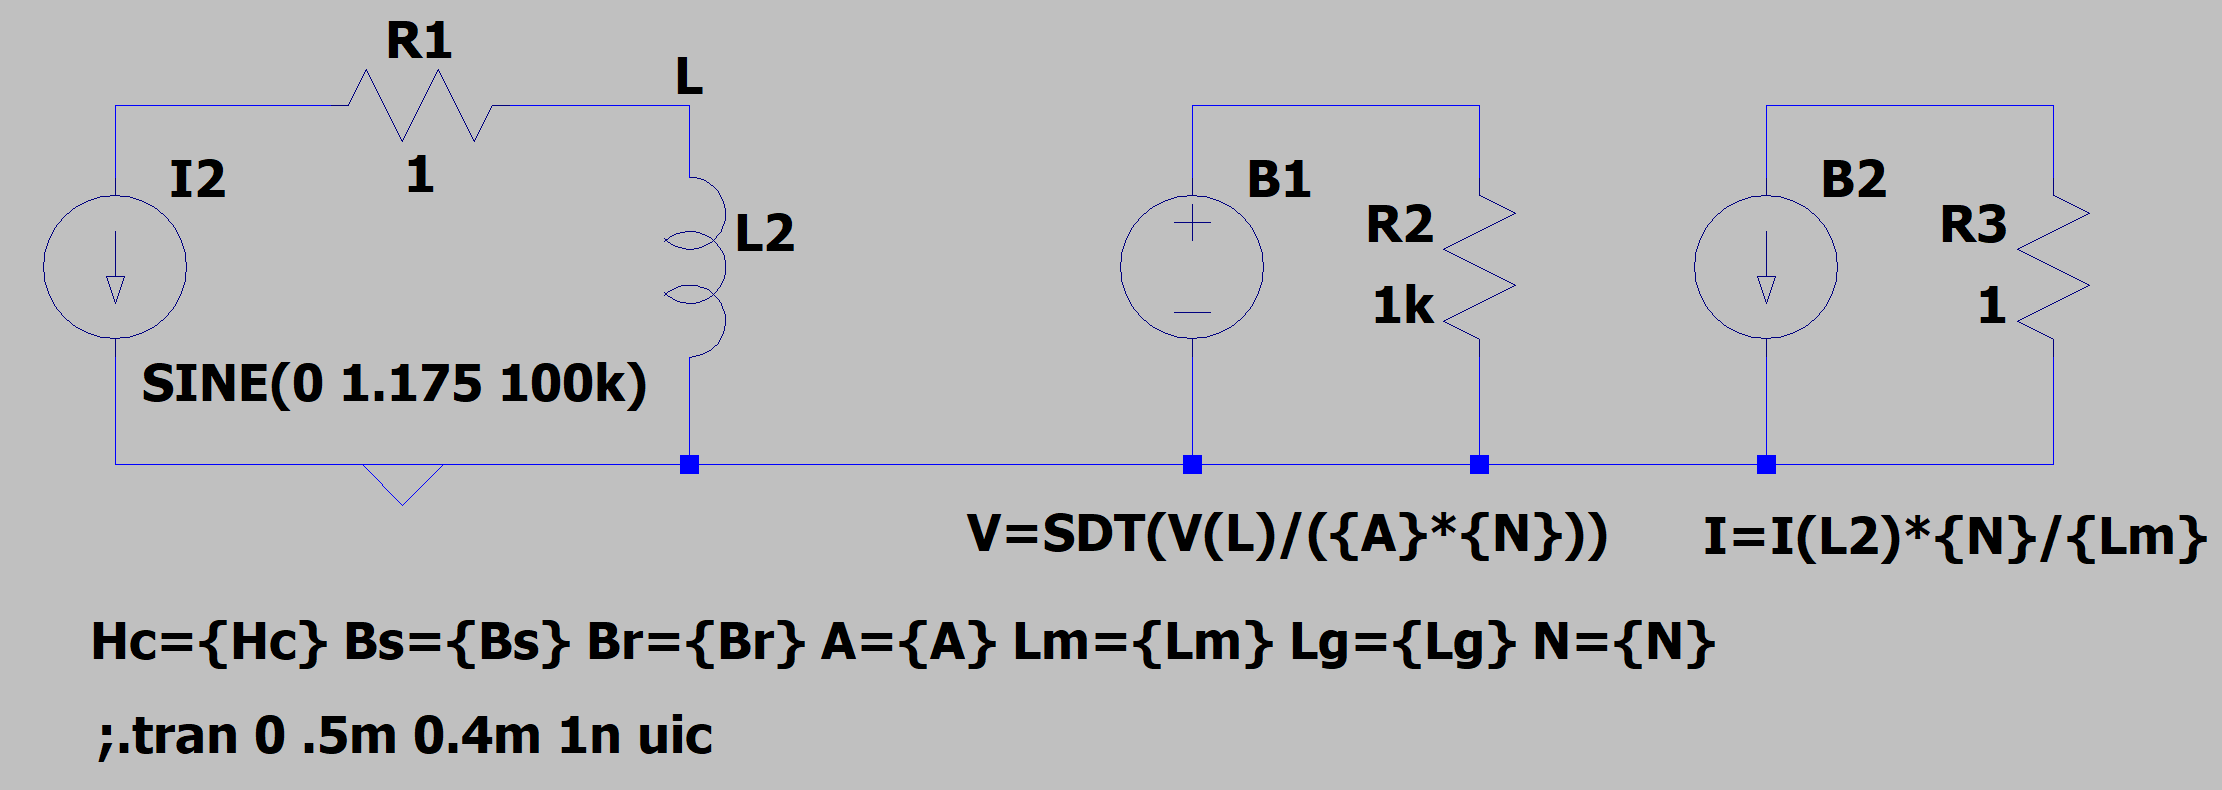
\includegraphics[width=.9\linewidth]{Bilder//Kapitel3/Hysteresis_Measurement_Setup_LTspice.png}
    \caption{Hysteresis measurement setup in LTspice}
    \label{fig:hysteresis_measurement_setup_in_LTspice}
\end{figure}
\subsection{Evaluation of the Hysteresis Model}
Plotting the voltage of the behavioural voltage source versus the current of the behavioural current source yields the simulated B-H curve shown in figure \ref{fig:hysteresis_comparison}. The hysteresis behaviour is represented well in the simulation. While the maximum B-field $B_{max}$ does differ from the expected value by \SI{50}{\milli\tesla}, the remnant B-field $B_r$ and coercivity $H_c$ only differ minimally from the input values, by \SI{3}{\micro\tesla} and \SI{0.13}{\A\per\m} respectively.
\begin{figure}[H]
    \begin{subfigure}[b]{0.50\textwidth}
        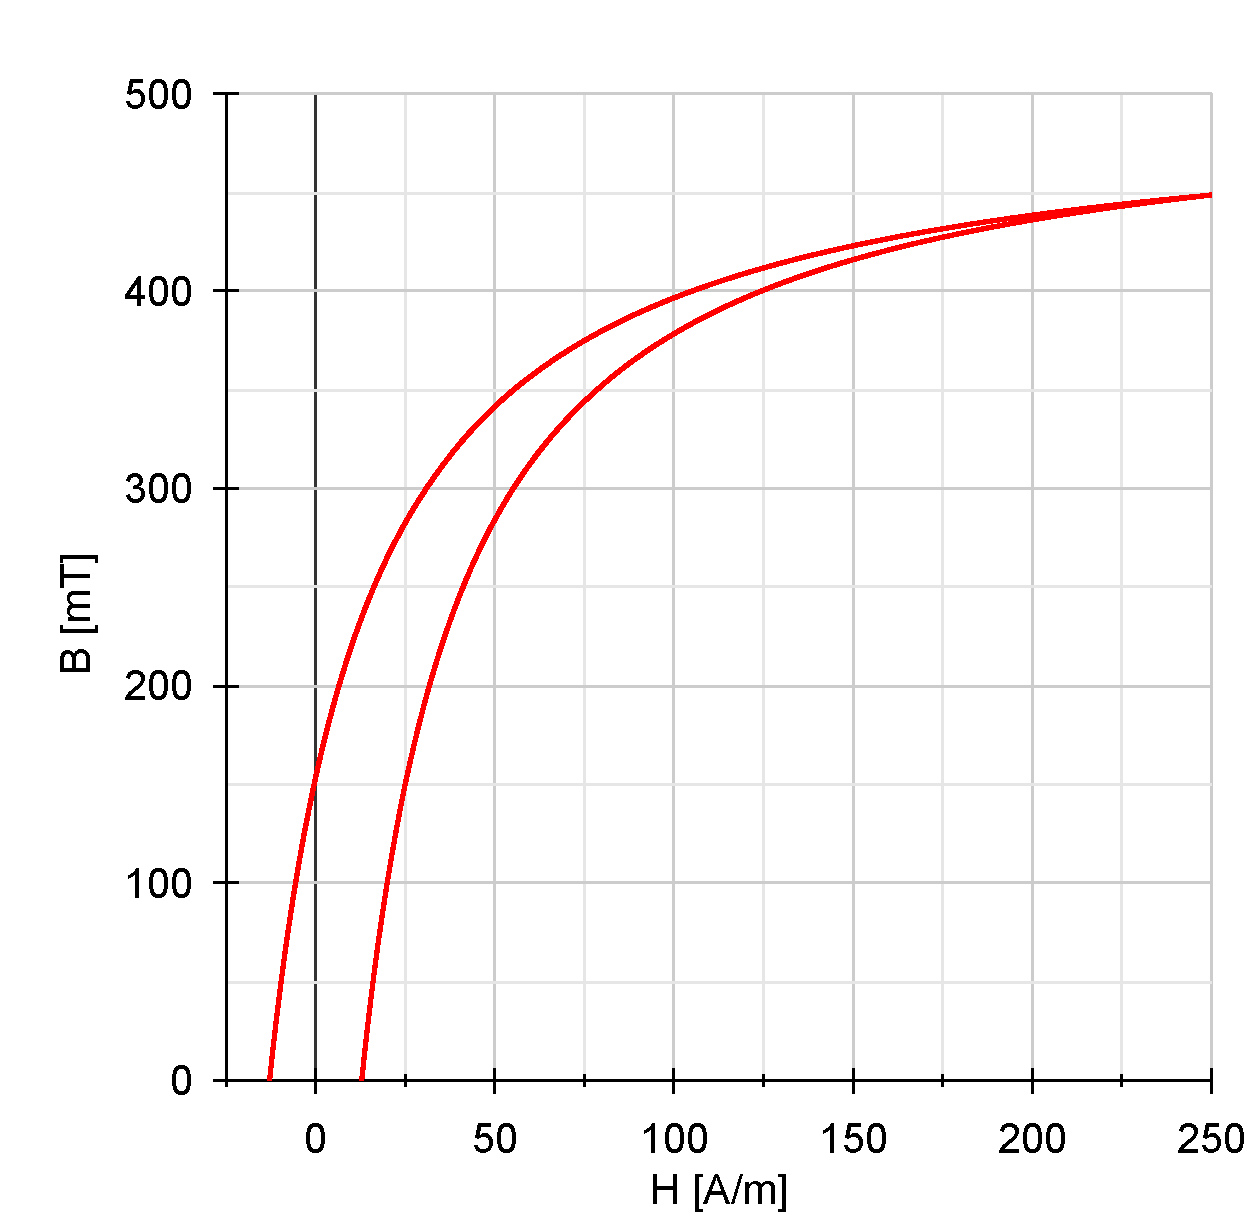
\includegraphics[width=\textwidth]{Bilder/Kapitel3/Hysteresis_LTspice_2.pdf}
        \caption{Simulated hysteresis curve}
    \end{subfigure}
    \begin{subfigure}[b]{0.49\textwidth}
        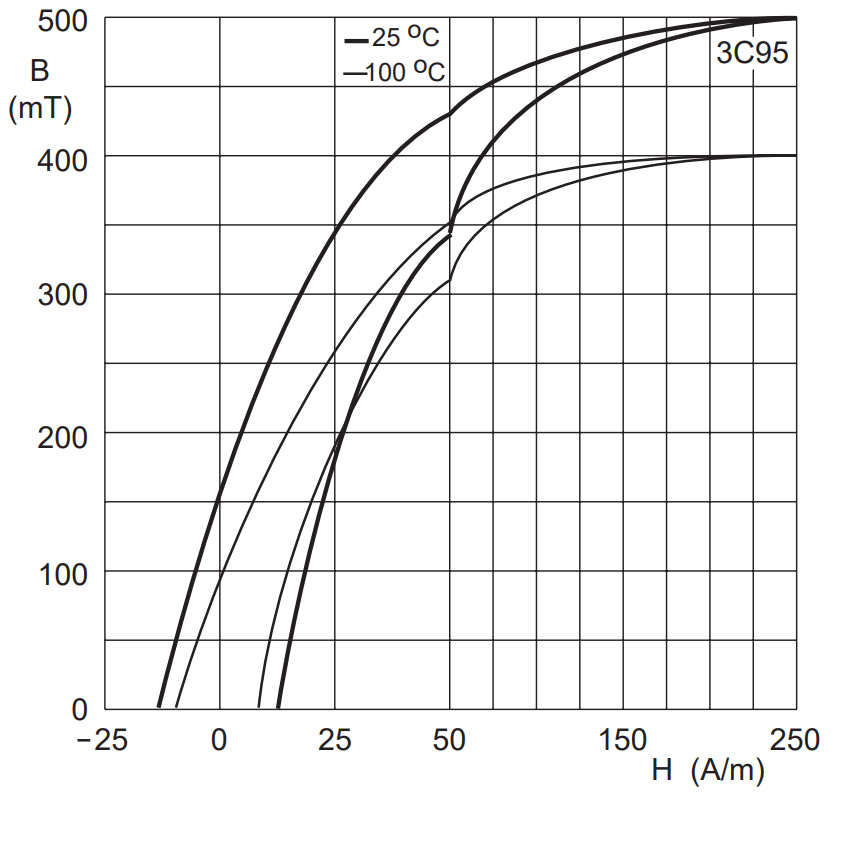
\includegraphics[width=\textwidth]{Bilder/Kapitel3/DataSheet_Hysteresis_Curve_2.png}
        \caption{Hysteresis given by the data sheet \cite{ferroxcubeProductSpecificationsCore2016}}
    \end{subfigure}
    \caption{Hysteresis comparison}
    \label{fig:hysteresis_comparison}							
\end{figure}
However, this does not yet validate the model. As the models main goal is to represent the effects of \ac{DC} bias while not in the saturation region, it has to be able to properly model the inductance of the inductor in the the low \ac{DC} bias range. For this the measurement approach used in section \ref{sec:saturation_behaviour_of_the_inductor} is used again on the custom inductor. First the physical inductor is measured and its saturation behaviour is extracted. The simulated inductor modeled through the hysteresis parameters then recreates the physical measurement. Their results are plotted in the graph \ref{fig:inductance_measured_and_simulatd}. 
\begin{figure}[H]
    \centering
    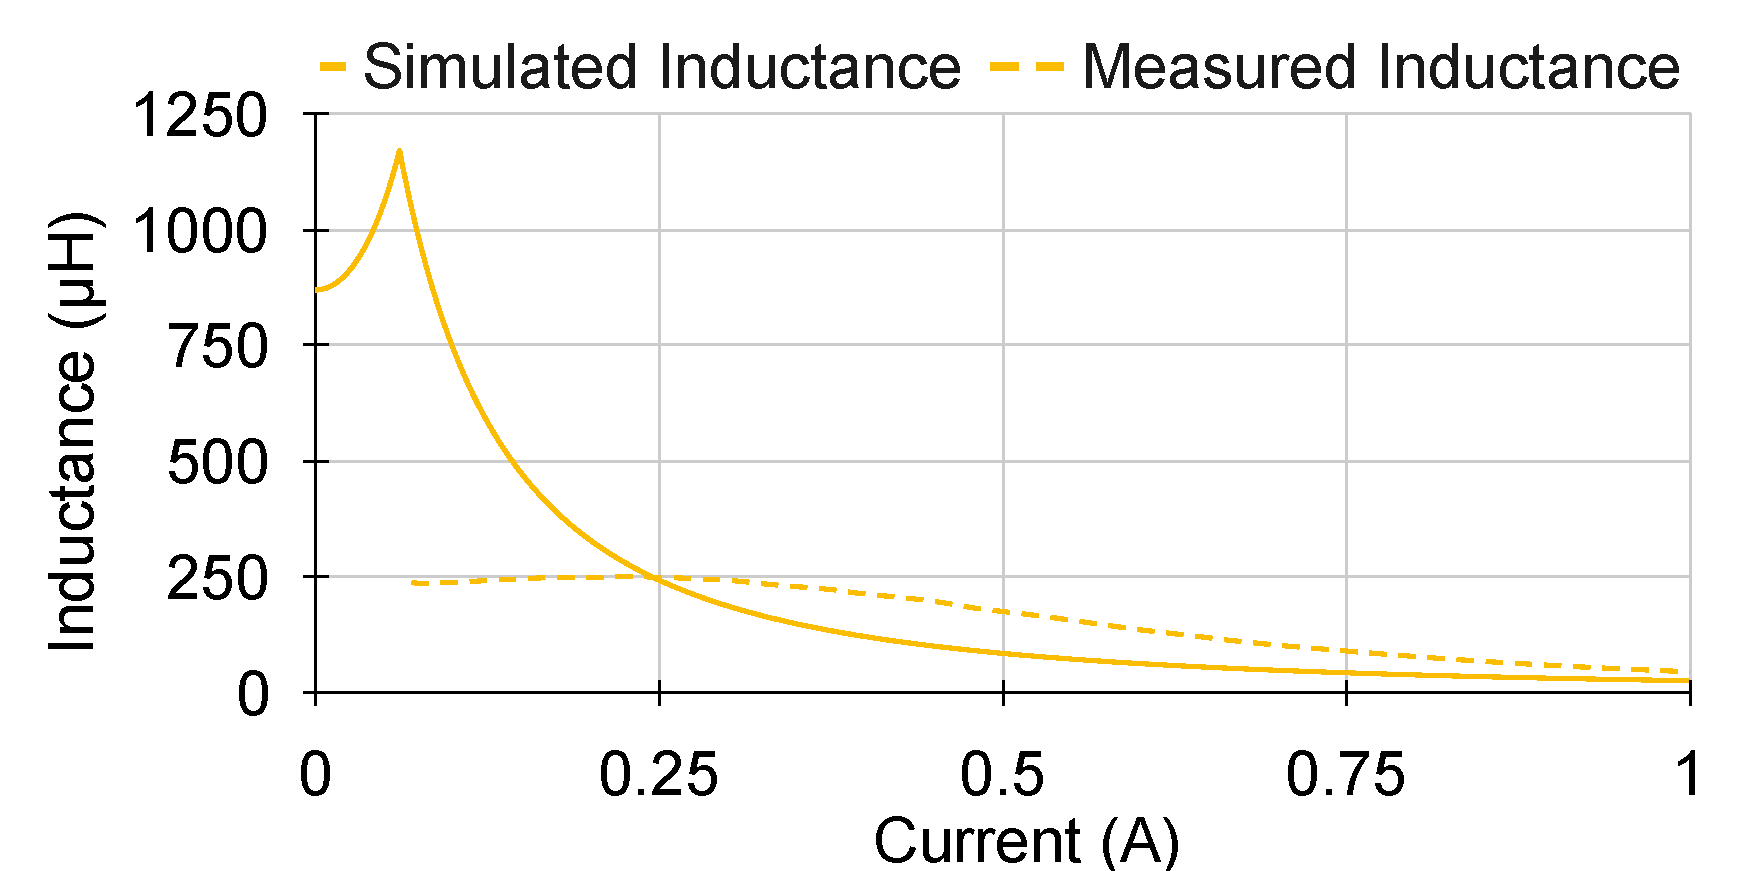
\includegraphics[width=.75\linewidth]{Bilder/Kapitel3/Saturation_Measured_and_Simulated_Hyst.pdf}
    \caption{Inductance measured and simulated}
    \label{fig:inductance_measured_and_simulatd}
\end{figure} 
Here the downside of the LTspice hysteresis modeling is shown. While demonstrating approximate hysteresis behaviour in figure \ref{fig:hysteresis_comparison}, the model is not able to recreate the inductance behaviour of the physical inductor, even though all measurement error from the hysteresis model has been removed. Because of this the hysteresis model is not implemented in the final inductor model.
